\documentclass[tikz,border=5pt]{standalone}
\begin{document}

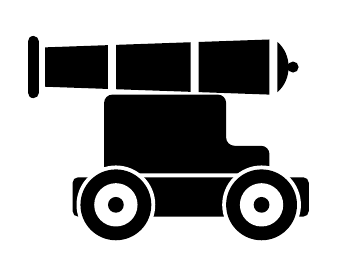
\begin{tikzpicture}[
    wheel/.pic={
        \fill[white] circle[radius=1cm];
        \fill[black] circle[radius=0.9cm];
        \fill[white] circle[radius=0.55cm];
        \fill[black] circle[radius=0.2cm];
    }
]   
    \begin{scope}[yshift=1.65cm]
        \fill[black] (-1.85,.25) -- (1,.35)-- (1,-.35) -- (-1.85,-.25) -- cycle;
        \fill[white] 
            (-1.05,-.5) rectangle ++(.1,1)
            (0,-.5) rectangle ++(.1,1)
        ;
        \draw[line cap=round,line width=4pt] (-2,-.325) -- (-2,.325);
        \coordinate (up) at (1.1,.32);
        \coordinate (down) at (1.1,-.32);
        \fill[black] (up) -- (down) to[bend right=50] (up) --cycle
                    (1.3,0) circle[radius=2pt];
    \end{scope}
    \fill[black,rounded corners=3pt] (-1.1,.3) -- (1,.3) -- ++(0,0.35) -- ++(-.55,0) -- ++(0,0.65) -| (-1.1,.3) -- cycle;
    \fill[black,rounded corners=2pt] (-1.5,-.25) rectangle (1.5,.25);
    \pic[scale=0.5] at (-.95,-.1) {wheel};
    \pic[scale=0.5] at (.9,-.1) {wheel};
\end{tikzpicture}

\end{document}